\documentclass[a4paper,12pt]{article}
\usepackage[letterpaper, landscape, left=1mm, right =1mm, top=3mm, bottom=2mm]{geometry}
\usepackage[table,xcdraw]{xcolor}
\usepackage[labelformat=empty]{caption}
\usepackage{booktabs,makecell,multirow,tabularx}
\usepackage{tikz}
\usetikzlibrary{shapes.geometric, arrows}

\begin{document}

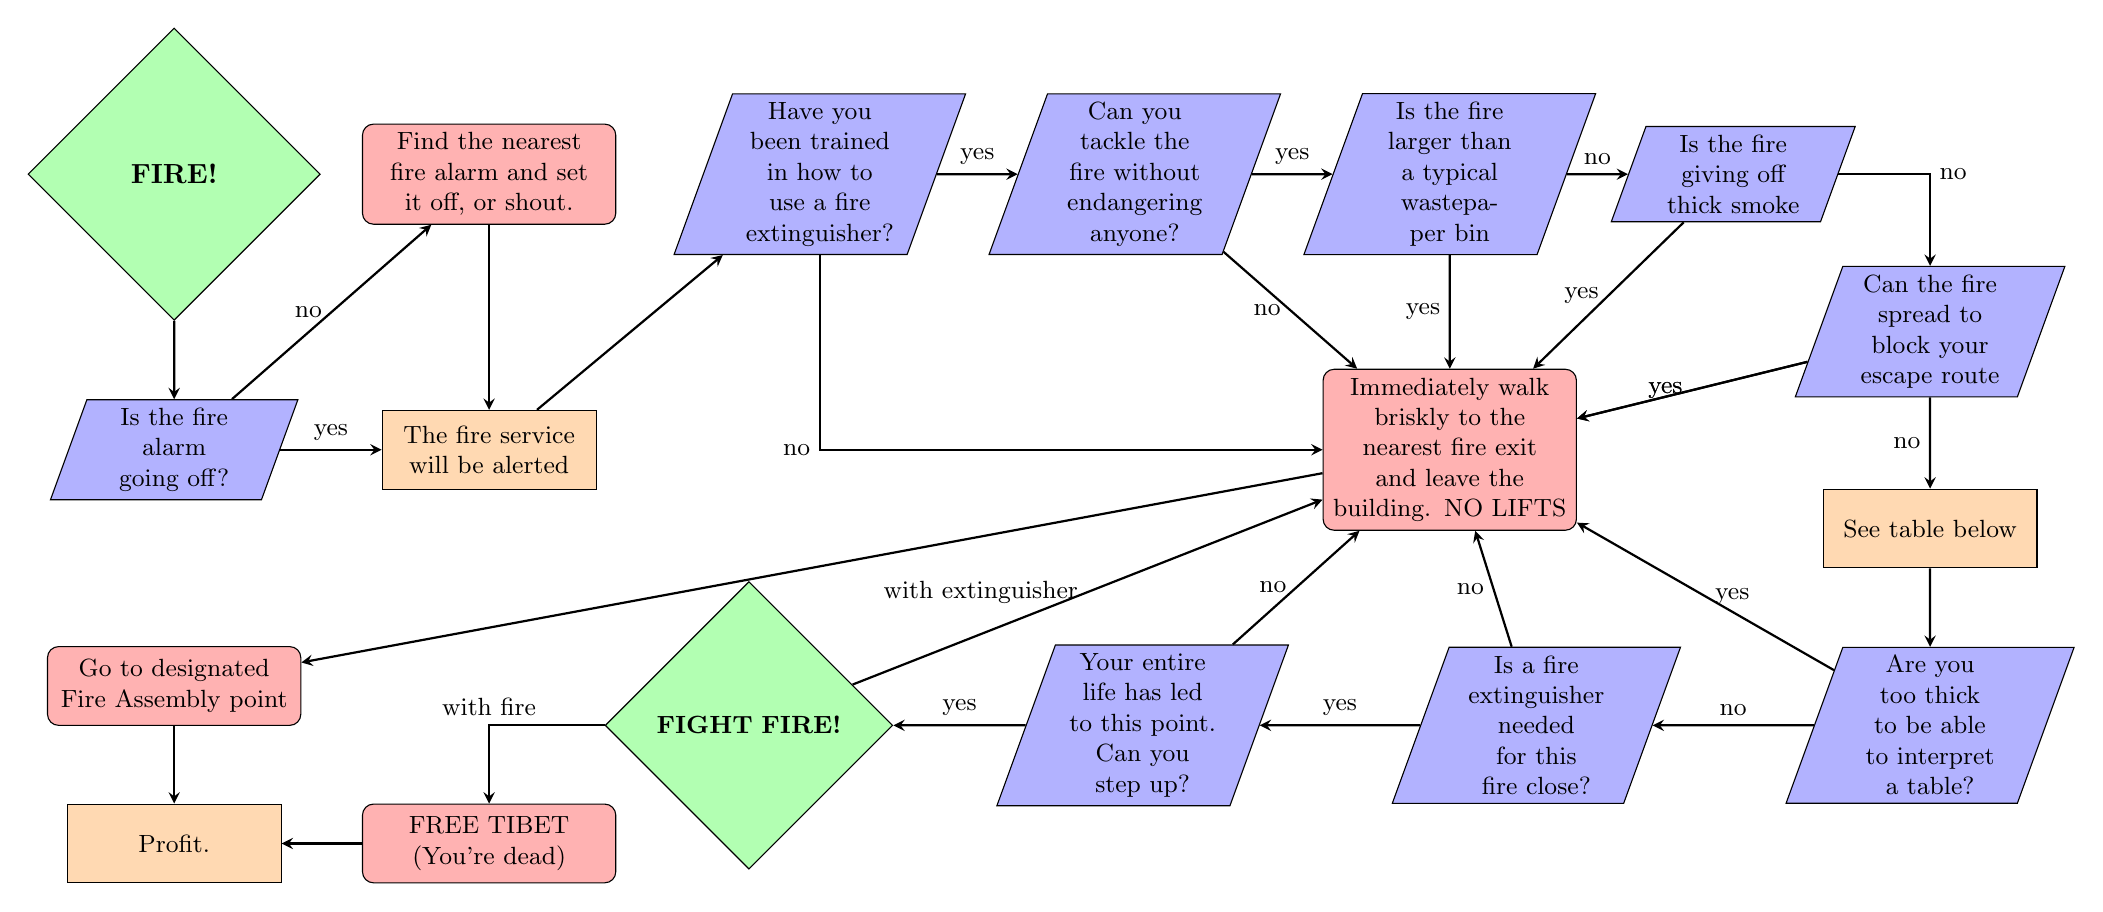
\begin{tikzpicture}[node distance=2cm]
\tikzstyle{startstop} =  [diamond, minimum width=0.2cm, minimum height=0.2cm, text centered,text width=3cm, draw=black, fill=green!30] 
\tikzstyle{question} = [trapezium, trapezium left angle=70, trapezium right angle=110, minimum width=2cm, minimum height=1cm, text centered, text width=2cm, draw=black, fill=blue!30]
\tikzstyle{process} = [rectangle, minimum width=2.5cm, minimum height=1cm, text centered, text width=2.5cm, draw=black, fill=orange!30]
\tikzstyle{action} = [rectangle, rounded corners, minimum width=3cm, minimum height=1cm,text centered, text width=3cm, draw=black, fill=red!30]
\tikzstyle{arrow} = [thick,->,>=stealth]

\node (start) [startstop] {\textbf{FIRE!}};
\small
\node (in1) [question, below of=start, yshift=-1.5cm] {Is the fire alarm going off?};
\node (act1) [action, right of=start, xshift =2cm] {Find the nearest fire alarm and set it off, or shout.};
\node (p1) [process, right of=in1, xshift=2cm] {The fire service will be alerted};
\node (in2) [question, right of=act1, xshift=2.2cm] {Have you been trained in how to use a fire extinguisher?};
\node (in3) [question, right of=in2, xshift=2cm] {Can you tackle the fire without endangering anyone?};
\node (in4) [question, right of=in3, xshift=2cm] {Is the fire larger than a typical wastepaper bin};
\node (in5) [question, right of=in4, xshift=1.6cm] {Is the fire giving off thick smoke};
\node (in6) [question, below of=in5, xshift=2.5cm] {Can the fire spread to block your escape route};
\node (p2) [process, below of=in6, yshift=-0.5cm] {See table below};
\node (act2) [action, below of=in4, yshift=-1.5cm] {Immediately walk briskly to the nearest fire exit and leave the building. NO LIFTS};
\node (act3) [action, below of=in1, yshift=-1cm] {Go to designated Fire Assembly point};
\node (in7) [question, below of=p2, yshift=-0.5cm] {Are you too thick to be able to interpret a table?};
\node (in8) [question, left of=in7, xshift=-3cm] {Is a fire extinguisher needed for this fire close?};
\node (in9) [question, left of=in8, xshift=-3cm] {Your entire life has led to this point. Can you step up?};
\node (end) [startstop, left of =in9, xshift=-3cm] {\textbf{FIGHT FIRE!}};
\node (act4) [action, below of=p1, yshift=-3cm] {FREE TIBET (You're dead)};
\node (p3) [process, left of=act4, xshift=-2cm] {Profit.};

\draw [arrow] (start) -- (in1);
\draw [arrow] (in1) -- node[anchor=south] {yes} (p1);
\draw [arrow] (in1) -- node[anchor=east] {no} (act1);
\draw [arrow] (act1) -- (p1);
\draw [arrow] (p1) -- (in2);
\draw [arrow] (in2) -- node[anchor=south] {yes} (in3);
\draw [arrow] (in2) |- node[anchor=east] {no} (act2);
\draw [arrow] (in3) -- node[anchor=south] {yes} (in4);
\draw [arrow] (in3) -- node[anchor=east] {no} (act2);
\draw [arrow] (in4) -- node[anchor=south] {no} (in5);
\draw [arrow] (in4) -- node[anchor=east] {yes} (act2);
\draw [arrow] (in5) -| node[anchor=west] {no} (in6);
\draw [arrow] (in5) -- node[anchor=east] {yes} (act2);
\draw [arrow] (in6) -- node[anchor=east] {no} (p2);
\draw [arrow] (in6) -- node[anchor=east] {yes} (act2);
\draw [arrow] (p2) -- (in7);
\draw [arrow] (in6) -- node[anchor=east] {yes} (act2);
\draw [arrow] (act2) -- (act3);
\draw [arrow] (in7) -- node[anchor=west] {yes} (act2);
\draw [arrow] (in7) -- node[anchor=south] {no} (in8);
\draw [arrow] (in8) -- node[anchor=east] {no} (act2);
\draw [arrow] (in8) -- node[anchor=south] {yes} (in9);
\draw [arrow] (in9) -- node[anchor=east] {no} (act2);
\draw [arrow] (in9) -- node[anchor=south] {yes} (end);
\draw [arrow] (end) -- node[anchor=east] {with extinguisher} (act2);
\draw [arrow] (end) -| node[anchor=south] {with fire} (act4);
\draw [arrow] (act4) -- (p3);
\draw [arrow] (act3) -- (p3);
\end{tikzpicture}


\begin{table}[h]
\centering
\caption{•}
\begin{tabular}{llllllll}
\cline{1-3}
\multicolumn{1}{|l|}{Key} & \multicolumn{1}{l|}{\cellcolor[HTML]{FE0000}} & \multicolumn{1}{l|}{Dangerous to attempt} &  &  &  &  &  \\ \cline{1-3} \cline{5-8} 
\multicolumn{1}{|l|}{} & \multicolumn{1}{l|}{\cellcolor[HTML]{F8FF00}} & \multicolumn{1}{l|}{Effective but slow} & \multicolumn{1}{l|}{} & \multicolumn{4}{l|}{\textbf{Extinguisher Type}} \\ \cline{1-3} \cline{5-8} 
\multicolumn{1}{|l|}{} & \multicolumn{1}{l|}{\cellcolor[HTML]{34FF34}} & \multicolumn{1}{l|}{Effective} & \multicolumn{1}{l|}{} & \multicolumn{1}{c|}{WATER} & \multicolumn{1}{c|}{FOAM} & \multicolumn{1}{c|}{POWDER} & \multicolumn{1}{c|}{CARBON DIOXIDE} \\ \cline{1-3} \cline{5-8} 
 &  &  & \multicolumn{1}{l|}{} & \multicolumn{1}{l|}{\begin{tabular}[c]{@{}l@{}}- Red\\ \\ - Hose\end{tabular}} & \multicolumn{1}{l|}{\begin{tabular}[c]{@{}l@{}}- Red \\ - Cream Strip\\ - Hose\end{tabular}} & \multicolumn{1}{l|}{\begin{tabular}[c]{@{}l@{}}- Red\\ - Blue Strip\\ - Hose\end{tabular}} & \multicolumn{1}{l|}{\begin{tabular}[c]{@{}l@{}}- Red\\ - Black Strip\\ - Conic Nuzzle\end{tabular}} \\ \cline{3-8} 
 & \multicolumn{1}{l|}{} & \multicolumn{1}{l|}{} & \multicolumn{1}{l|}{Wood/Paper} & \multicolumn{1}{l|}{\cellcolor[HTML]{32CB00}\textit{}} & \multicolumn{1}{l|}{\cellcolor[HTML]{F8FF00}\textit{\begin{tabular}[c]{@{}l@{}}Slow to cover\\ the gaps and\\ smother fire\end{tabular}}} & \multicolumn{1}{l|}{\cellcolor[HTML]{FE0000}\textit{\begin{tabular}[c]{@{}l@{}}Won't put out\\ the fire\end{tabular}}} & \multicolumn{1}{l|}{\cellcolor[HTML]{F8FF00}\textit{\begin{tabular}[c]{@{}l@{}}Slow to push out the\\ air and doesn't cool \\ wood/paper effectively\end{tabular}}} \\ \cline{4-8} 
 & \multicolumn{1}{l|}{} & \multicolumn{1}{l|}{} & \multicolumn{1}{l|}{Electric} & \multicolumn{1}{l|}{\cellcolor[HTML]{FE0000}\textit{\begin{tabular}[c]{@{}l@{}}Possible\\ Electrocution\end{tabular}}} & \multicolumn{1}{l|}{\cellcolor[HTML]{FE0000}\textit{\begin{tabular}[c]{@{}l@{}}Possible\\ Electrocution\end{tabular}}} & \multicolumn{1}{l|}{\cellcolor[HTML]{F8FF00}\textit{\begin{tabular}[c]{@{}l@{}}Requires a lot\\ of powder\end{tabular}}} & \multicolumn{1}{l|}{\cellcolor[HTML]{32CB00}\textit{}} \\ \cline{4-8} 
 & \multicolumn{1}{l|}{} & \multicolumn{1}{l|}{} & \multicolumn{1}{l|}{\begin{tabular}[c]{@{}l@{}}Chip Pan\\ (Contained \\ Liquid/Fat)\end{tabular}} & \multicolumn{1}{l|}{\cellcolor[HTML]{FE0000}\textit{\begin{tabular}[c]{@{}l@{}}Possible fat/oil \\ explosion\end{tabular}}} & \multicolumn{1}{l|}{\cellcolor[HTML]{32CB00}\textit{}} & \multicolumn{1}{l|}{\cellcolor[HTML]{F8FF00}\textit{\begin{tabular}[c]{@{}l@{}}Can get saturated\\ with oil and sink\end{tabular}}} & \multicolumn{1}{l|}{\cellcolor[HTML]{32CB00}\textit{}} \\ \cline{4-8} 
 & \multicolumn{1}{l|}{} & \multicolumn{1}{l|}{\multirow{-4}{*}{\textbf{Fire Type}}} & \multicolumn{1}{l|}{Spilled Liquid} & \multicolumn{1}{l|}{\cellcolor[HTML]{FE0000}\textit{Spreads the fire}} & \multicolumn{1}{l|}{\cellcolor[HTML]{32CB00}\textit{}} & \multicolumn{1}{l|}{\cellcolor[HTML]{32CB00}\textit{}} & \multicolumn{1}{l|}{\cellcolor[HTML]{F8FF00}\textit{\begin{tabular}[c]{@{}l@{}}Areas not being sprayed \\ are prone to re-ignition\end{tabular}}} \\ \cline{3-8} 
\end{tabular}
\end{table}
\end{document}
